\documentclass[xetex,serif]{beamer}
\usetheme{Warsaw}


\usepackage{amsmath, amssymb, color, url, amsthm, amsfonts,hyperref}
\usepackage{tabularx}
\usepackage{amstext}
\usepackage{algorithm2e}
\usepackage{graphicx}
\usepackage{wrapfig}
\usepackage{hhline}
\usepackage{color}
\usepackage[english]{babel}
\usepackage[utf8]{inputenc}
\usepackage{lipsum}
\usepackage [autostyle, english = american]{csquotes}
\MakeOuterQuote{"}


\setbeamercolor{postit}{fg=white,bg=blue}
\setbeamerfont{page number in head/foot}{size=\tiny}
\setbeamertemplate{footline}[frame number]
\setbeamerfont{frametitle}{size=\small}

\usepackage{xltxtra}
\XeTeXlinebreaklocale "th"
\defaultfontfeatures{Scale=1.4}
\setmainfont[Script=Thai]{TH SarabunPSK}

\title{\textbf{Cyber Warfare}}
\author{\textbf{น.ท.กรกช วิไลลักษณ์}}
\institute[]{โรงเรียนเสนาธิการทหารเรือ}
\date{} 

\begin{document}

\begin{frame}
\titlepage
\end{frame}

\begin{frame}
\tableofcontents[
  currentsection,
  sectionstyle=show,
  subsectionstyle=show/show/hide,
]
\end{frame}

\frame{\frametitle{วัตถุประสงค์การเรียนรู้}
	\begin{beamercolorbox}[rounded=true,wd=\linewidth]{postit}
		เมื่อสิ้นสุดการบรรยาย นทน.ฯ ควร
	\end{beamercolorbox}
	\begin{itemize}
		\item เข้าใจหลักการปฏิบัติการไซเบอร์
		\item เข้าใจหลักการรักษาความมั่นคงปลอดภัยทรัพยาการสารสนเทศและการสื่อสาร
		\item เข้าใจความเกี่ยวข้องกันของ "PPT" ในปฏิบัติการไซเบอร์
		\item ประยุกต์ใช้ความรู้ที่ได้รับอย่างเหมาะสม
	\end{itemize}
}



\section{สงครามไซเบอร์}
\frame{\frametitle{\null}
	\begin{beamercolorbox}[rounded=true,wd=\linewidth]{postit}
	\centering
		Cyber Warfare
	\end{beamercolorbox}
	%\begin{itemize}
	%	\item 
	%	\item 
	%\end{itemize}
}

\subsection{The Cyberspace Battlefield}
\frame{\frametitle{Clausewitz: On War}
	%\begin{beamercolorbox}[rounded=true,wd=\linewidth]{postit}
	% 
	%\end{beamercolorbox}
	\begin{figure}[!htbp]
		\centering
		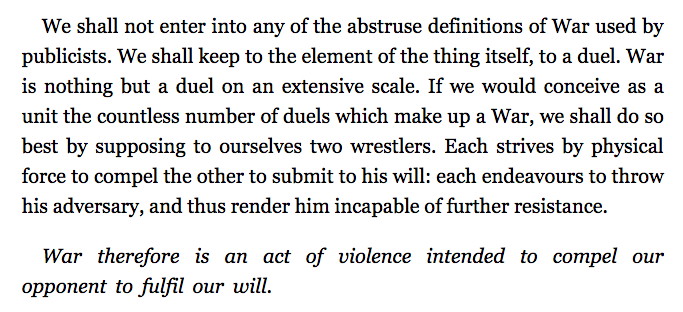
\includegraphics[height=.5\textheight, width=\textwidth]{figures/onwar.png}
	\end{figure}
	%\begin{itemize}
	%	\item 
	%	\item 
	%\end{itemize}
}

\frame{\frametitle{\null}
	%\begin{beamercolorbox}[rounded=true,wd=\linewidth]{postit}
	%
	%\end{beamercolorbox}
	\centering
	\begin{figure}[!htbp]
		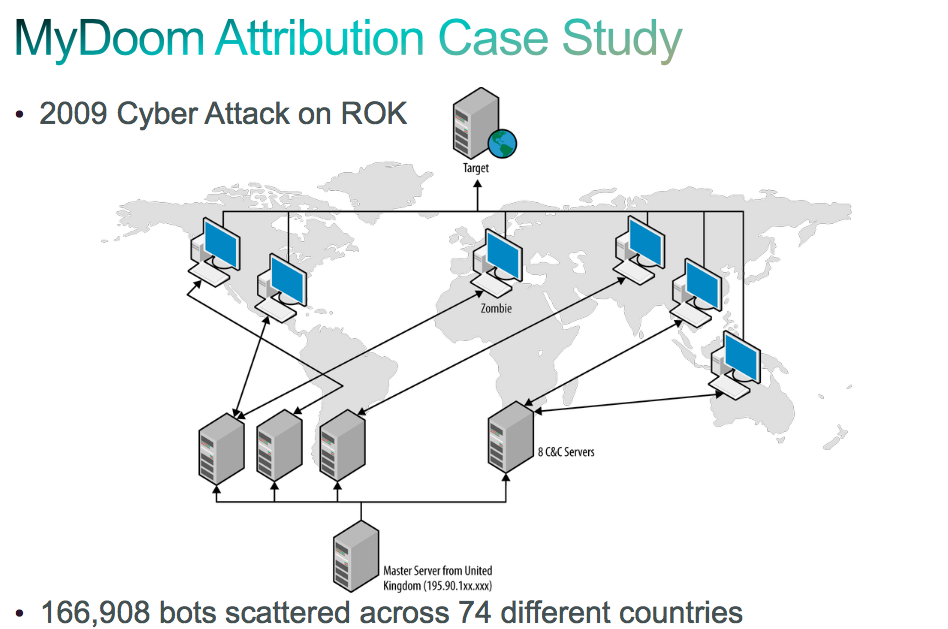
\includegraphics[height=.75\textheight, width=\textwidth]{figures/2009_attack_to_rok.png}
	\end{figure}
}

\frame{\frametitle{\null}
	%\begin{beamercolorbox}[rounded=true,wd=\linewidth]{postit}
	%
	%\end{beamercolorbox}
	\centering
	\begin{figure}[!htbp]
		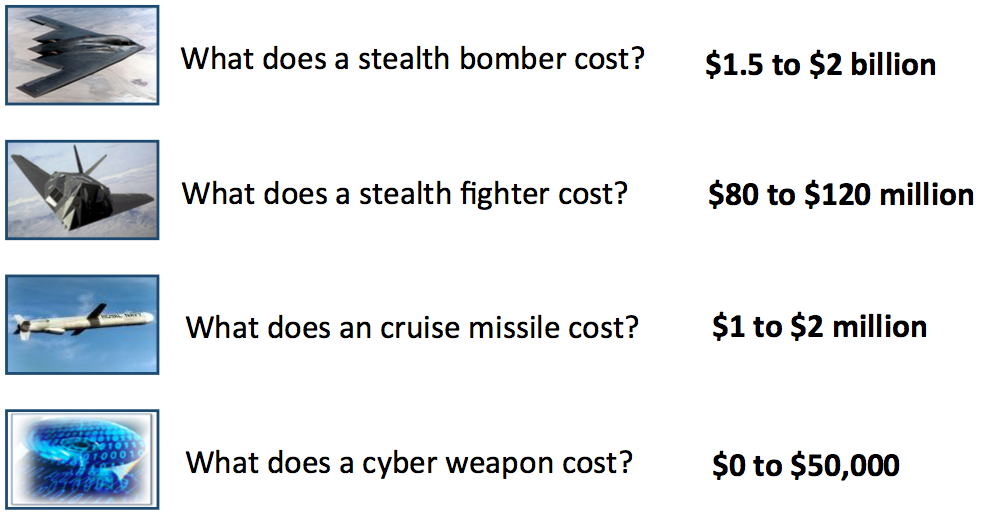
\includegraphics[height=.75\textheight, width=\textwidth]{figures/cyber_weapons.png}
	\end{figure}
}

\frame{\frametitle{What is cyber warfare?}
	%\begin{beamercolorbox}[rounded=true,wd=\linewidth]{postit}
	%
	%\end{beamercolorbox}
	\begin{itemize}
		\item Information Operation
		\item ปฏิบัติการทางทหารสาขาหนึ่งของปฏิบัติการข่าวสาร (Information warfare)
		\item มุ่งทำลาย CIA ของฝ่ายตรงข้าม
		\item Symmetric or Asymmetric
		\item JP 3-13 Information Operation
	\end{itemize}
}

\frame{\frametitle{เหตุใดจึงต้องเรียนรู้?}
	%\begin{beamercolorbox}[rounded=true,wd=\linewidth]{postit}
	%
	%\end{beamercolorbox}
	\begin{itemize}
		\item \textbf{D} iplomatic
		\item \textbf{I} nformation
		\item \textbf{M} ilitary
		\item \textbf{E} conomy
	\end{itemize}
	\centering
	\begin{beamercolorbox}[rounded=true,wd=\linewidth]{postit}
		Cyber space is a battlefield of the Internet and the ubiquitous nature of cyber conflicts being enmeshed into the physical battle field.
	\end{beamercolorbox} 
}


\frame{\frametitle{คุณลักษณะสนามรบ: ขอบเขตของสนามรบ}
	%\begin{beamercolorbox}[rounded=true,wd=\linewidth]{postit}
	%
	%\end{beamercolorbox}
	\begin{itemize}
		\item ขอบเขตเชิงตรรกะ (Logical boundary)
		\item ขอบเขตเชิงกายภาพ (Physical boundary)
		\item ขอบเขตเชิงการบริหารจัดการ (Organizational boundary)
	\end{itemize}
}

\frame{\frametitle{คุณลักษณะสนามรบ: ขอบเขตของสนามรบ(Cont.)}
	\begin{beamercolorbox}[rounded=true,wd=\linewidth]{postit}
		ขอบเขตเชิงตรรกะ (Logical boundary)
	\end{beamercolorbox}
	%\begin{itemize}
	%	\item 
	%\end{itemize}
	\begin{figure}[!htbp]
		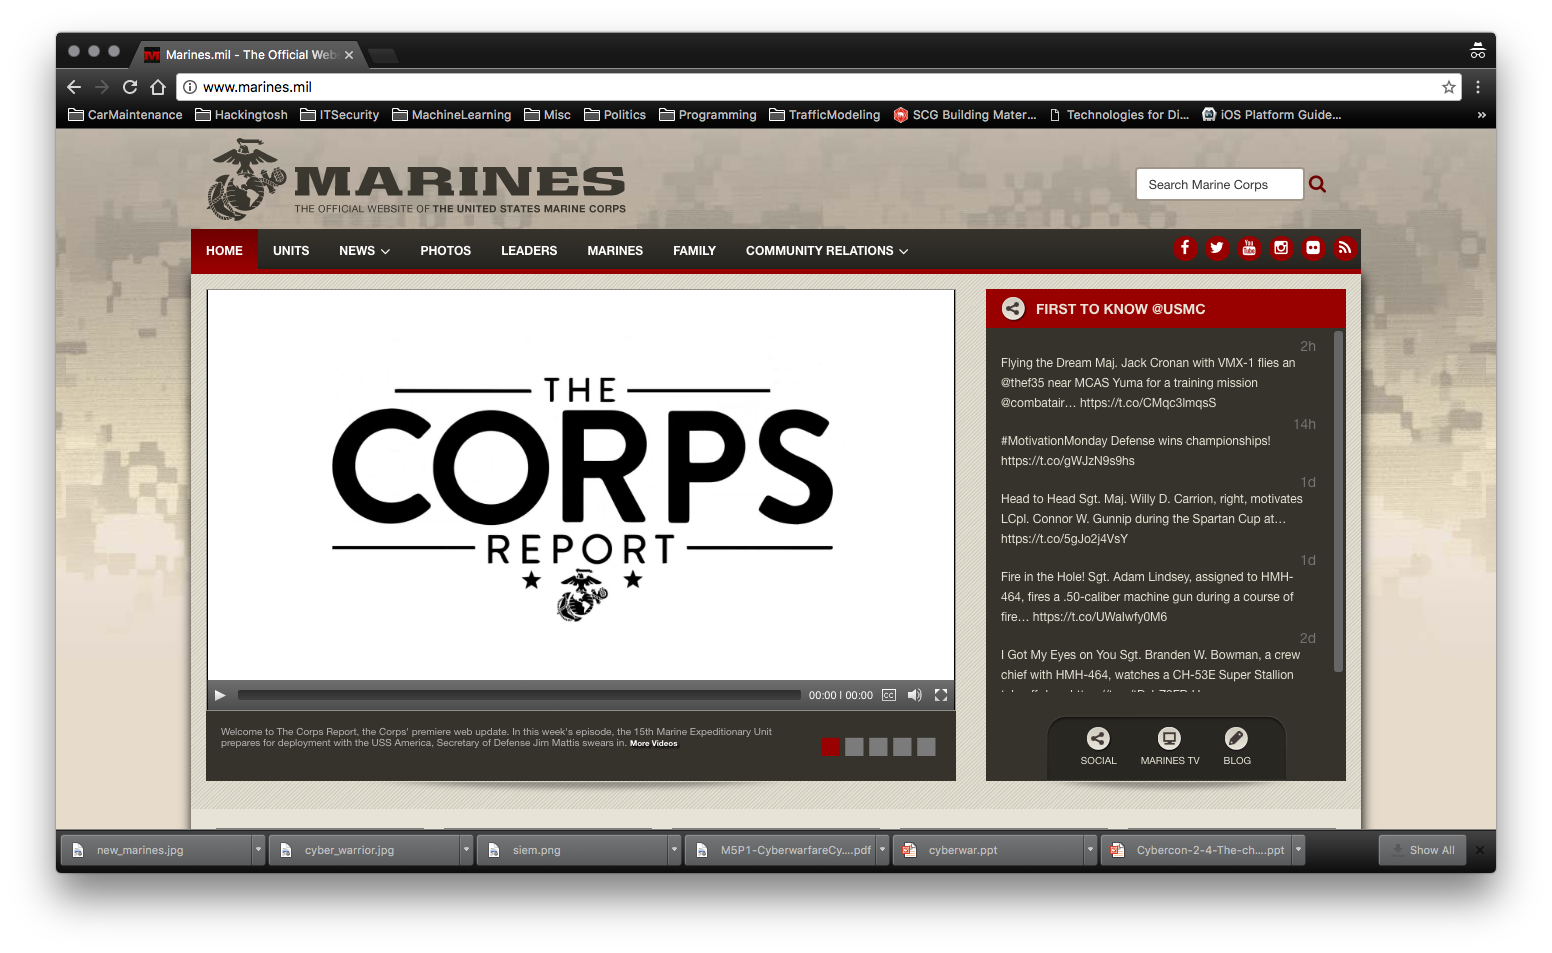
\includegraphics[height=.75\textheight, width=\textwidth]{figures/logical_boundary.png}
	\end{figure}
}


\frame{\frametitle{คุณลักษณะสนามรบ: ขอบเขตของสนามรบ(Cont.)}
	\begin{beamercolorbox}[rounded=true,wd=\linewidth]{postit}
		ขอบเขตเชิงกายภาพ (Physical boundary)
	\end{beamercolorbox}
	%\begin{itemize}
	%	\item 
	%\end{itemize}
	\begin{figure}[!htbp]
		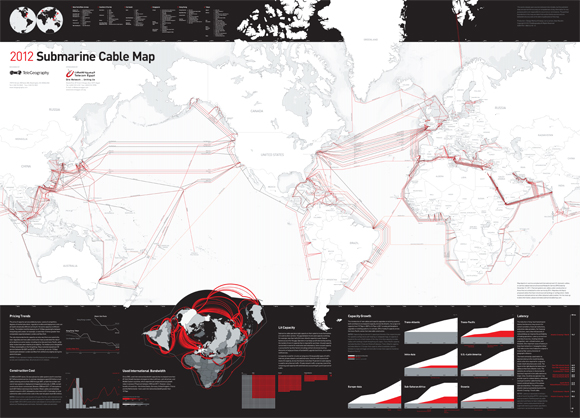
\includegraphics[height=.65\textheight, width=\textwidth]{figures/submarine-cable-map-2012-m.jpg}
	\end{figure}
}


\frame{\frametitle{คุณลักษณะสนามรบ: ขอบเขตของสนามรบ(Cont.)}
	\begin{beamercolorbox}[rounded=true,wd=\linewidth]{postit}
		ขอบเขตเชิงการบริหารจัดการ
	\end{beamercolorbox}
	%\begin{itemize}
	%	\item 
	%	\item 
	%\end{itemize}
	\centering
	\begin{figure}[!htbp]
		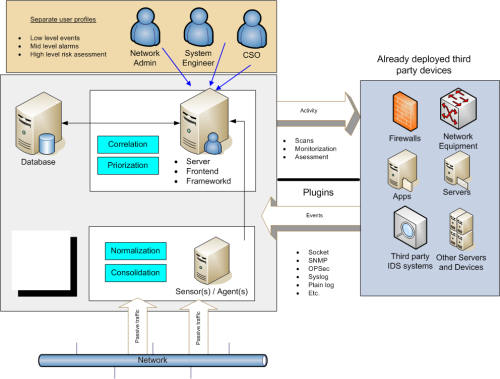
\includegraphics[height=.65\textheight, width=\textwidth]{figures/siem.png}
	\end{figure}
}


\subsection{Cyber Doctrine}
\frame{\frametitle{Conventional War Fighting}
	%\begin{beamercolorbox}[rounded=true,wd=\linewidth]{postit}
	%Covered topics
	%\end{beamercolorbox}
	\begin{itemize}
		\item การปฏิบัติ (เทคนิคการโจมตี) จะแตกต่างกันออกไปขึ้นอยู่กับระดับของสงคราม
		\begin{itemize}
			\item Strategic
			\item Operational
			\item Tactical
		\end{itemize}
		\item มุ่งทำลาย COG ของเป้าหมายเชิงยุทธศาสตร์
		\begin{itemize}
			\item กำลังทางบก
			\item กำลังทางอากาศ
			\item กำลังทางเรือ
			\item โครงสร้างพื้นฐานที่เกี่ยวข้องกับการสื่อสารและโทรคมนาคม
		\end{itemize}
	\end{itemize}
}

\frame{\frametitle{Cyber warfare}
	%\begin{beamercolorbox}[rounded=true,wd=\linewidth]{postit}
	%Covered topics
	%\end{beamercolorbox}
	\begin{itemize}
	\item มุ่งทำลาย CIA ของเป้าหมายเชิงยุทธศาสตร์
	\begin{itemize}
		\item ค้นหาช่องโหว่ของโครงสร้างพื้นฐานระบบสารสนเทศและการสื่อสาร
		\item ปฏิบัติการข้อมูลข่าวสาร PSYOPS, Disinformation, Diversionary
		\item โจมตีผสมผสานกับ Electronic Attack Vectors อื่นๆ
		\item รบกวนระบบตรวจจับต่างๆ และทำลายโครงสร้างพื้นฐานการควบคุมบังคับบัญชา
	\end{itemize}
\end{itemize}
}

\subsection{Cyber Warriors}

\frame{\frametitle{นักรบ}
	%\begin{beamercolorbox}[rounded=true,wd=\linewidth]{postit}
	%Covered topics
	%\end{beamercolorbox}
	%Covered topics
%\end{beamercolorbox}
	\centering
	\begin{figure}[!htbp]
		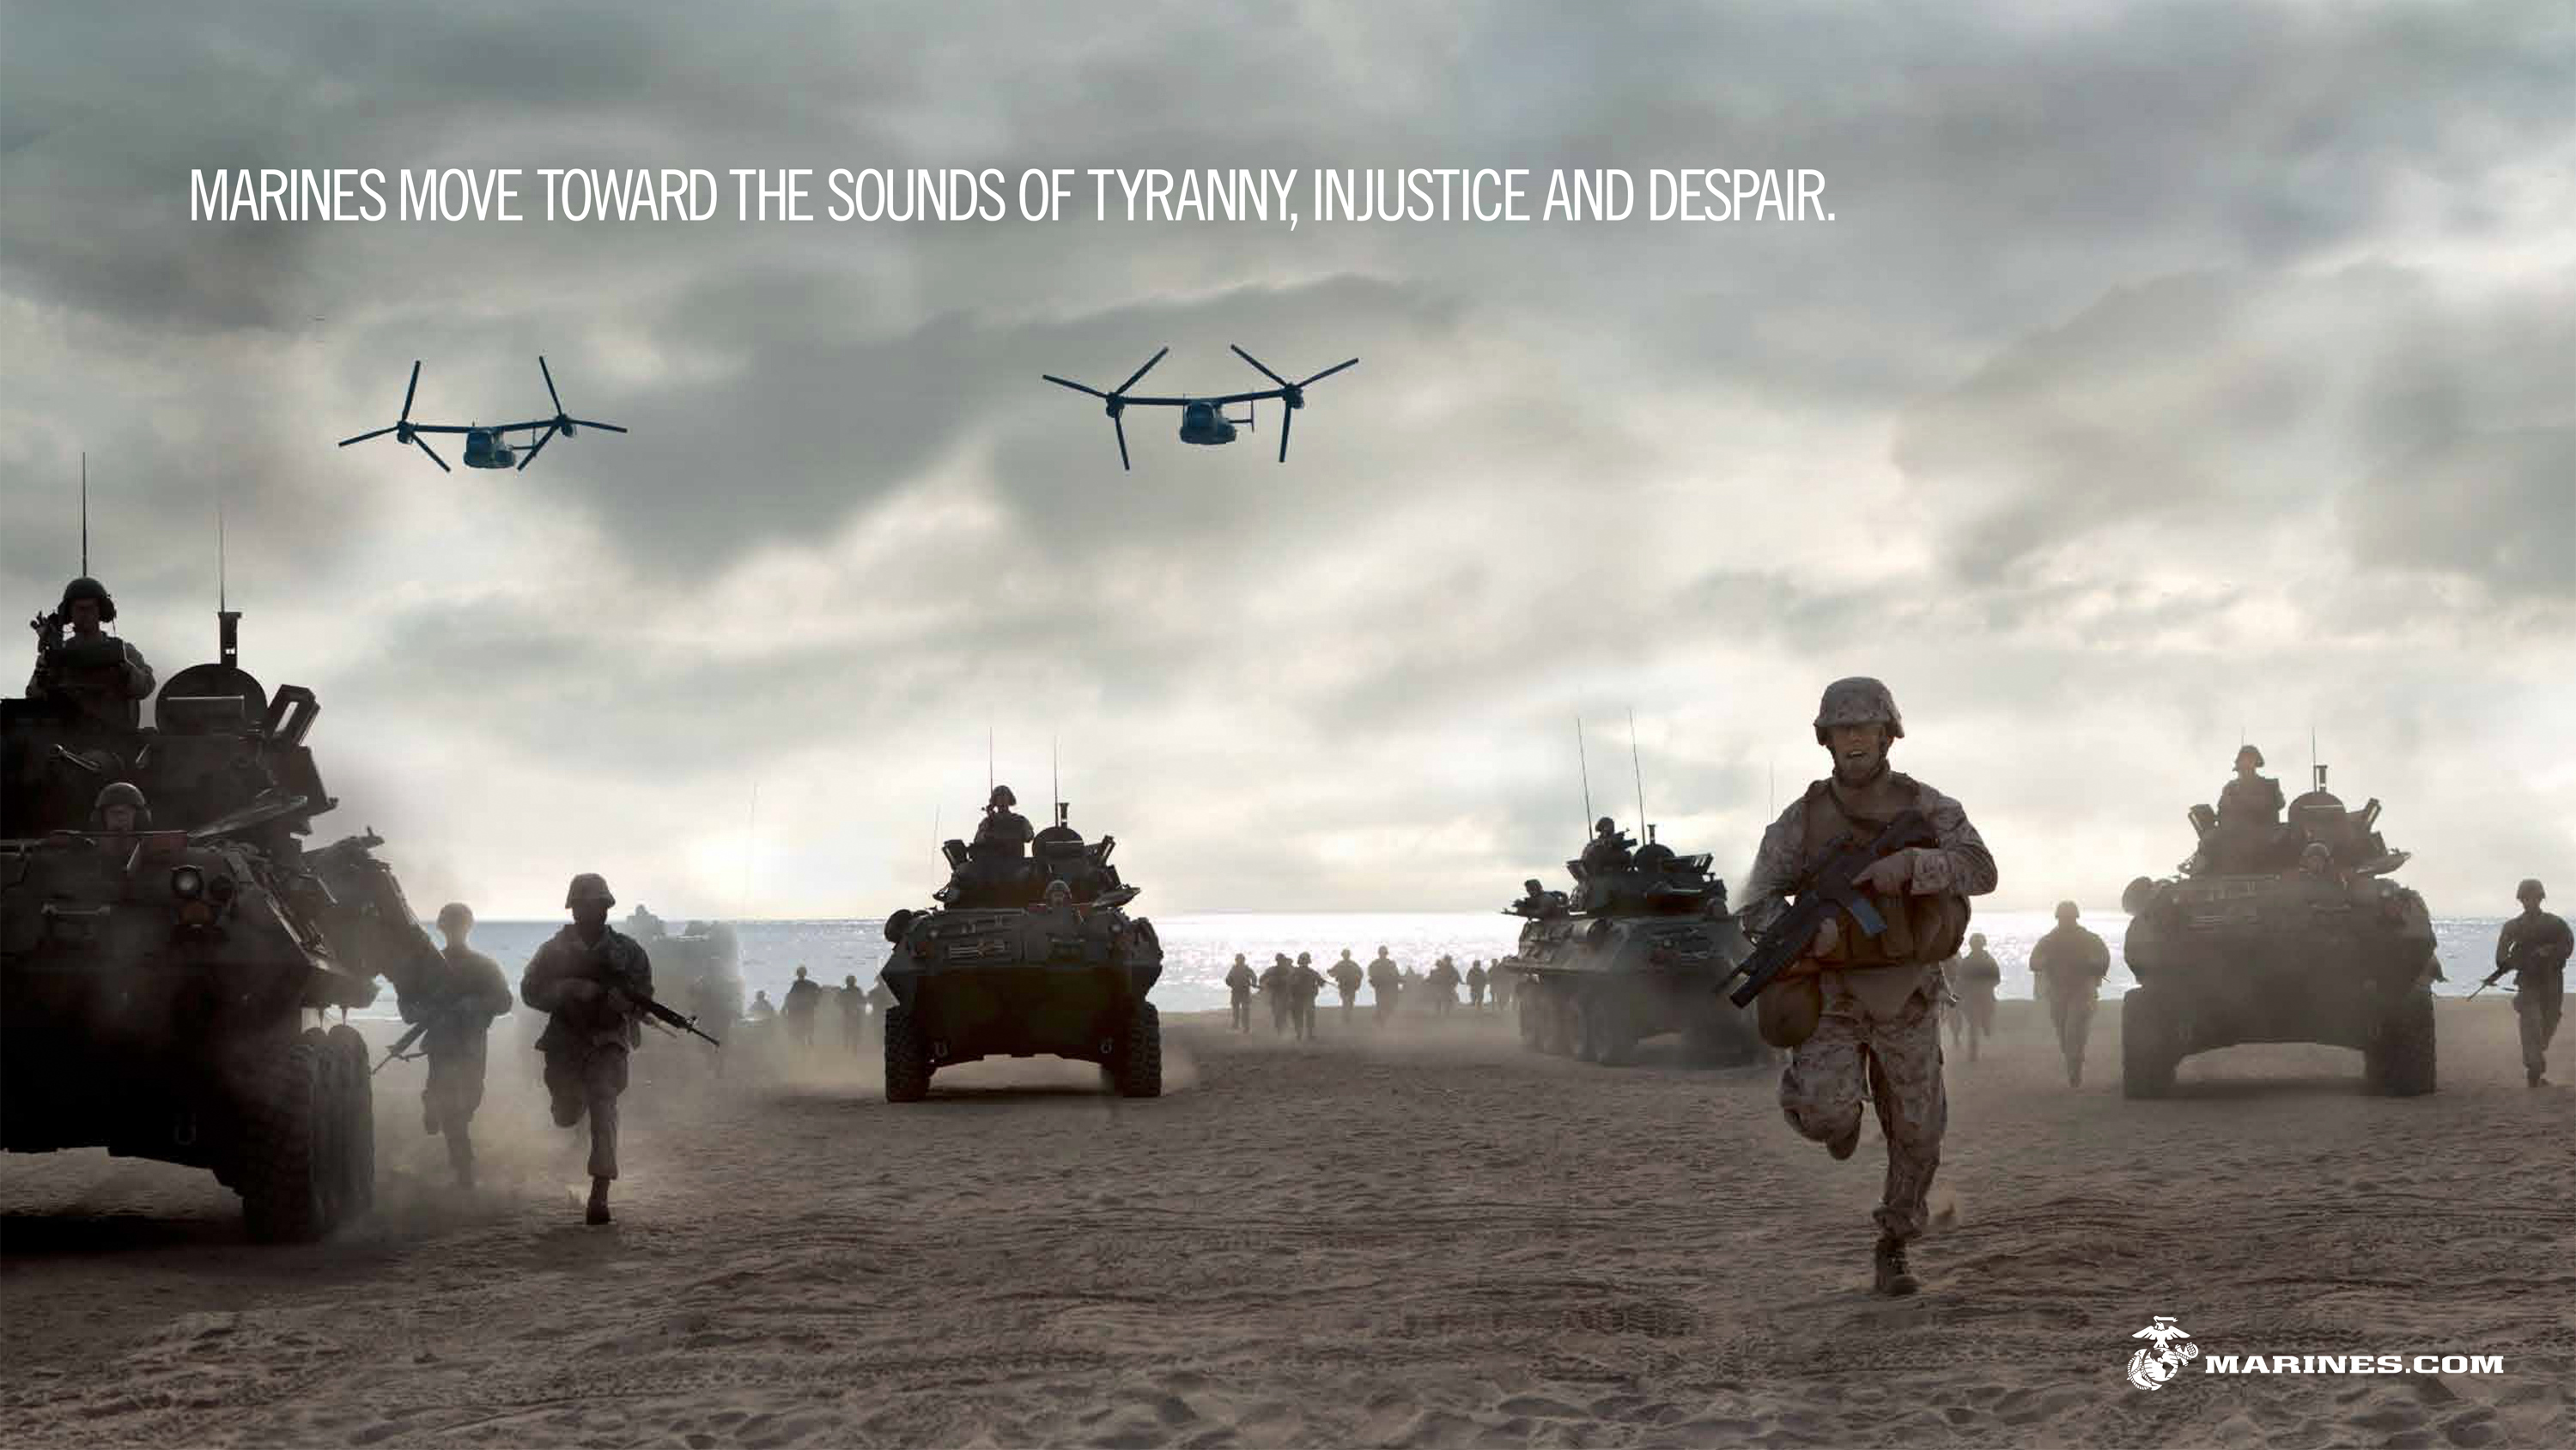
\includegraphics[height=.75\textheight, width=\textwidth]{figures/new_marines.jpg}
	\end{figure}
}

\frame{\frametitle{นักรบไซเบอร์}
	%\begin{beamercolorbox}[rounded=true,wd=\linewidth]{postit}
	%Covered topics
	%\end{beamercolorbox}
	\centering
	\begin{figure}[!htbp]
		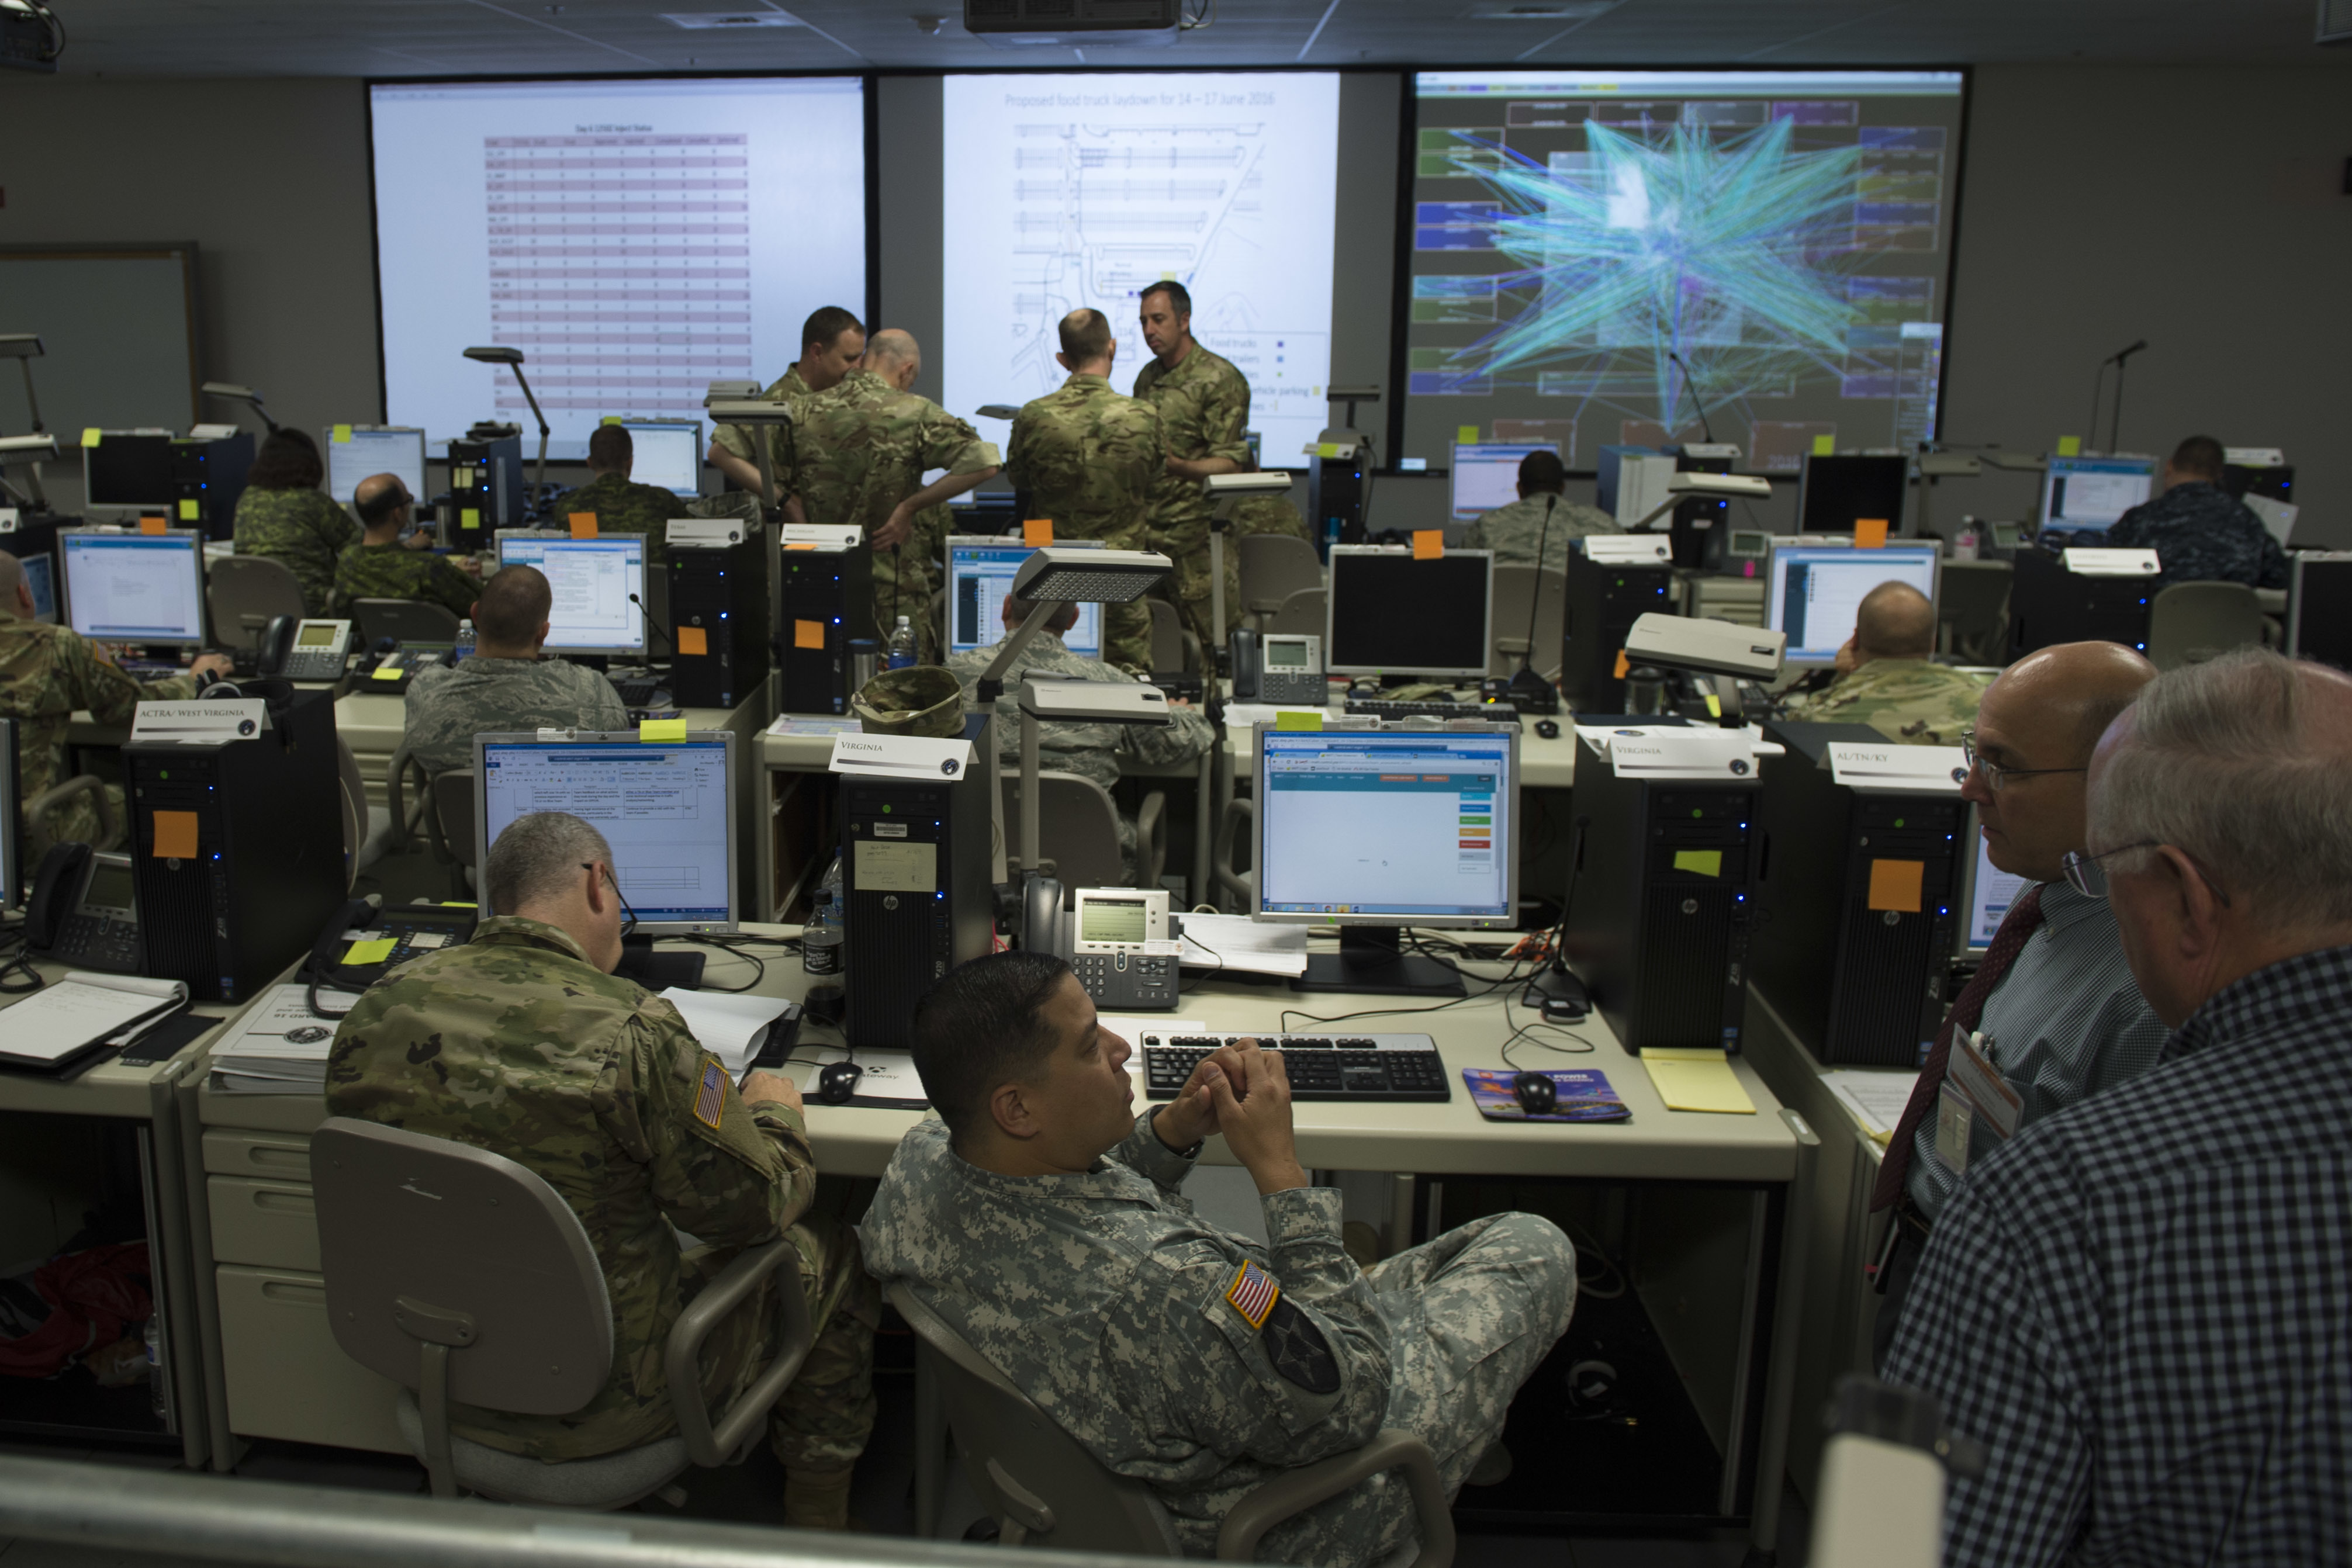
\includegraphics[height=.75\textheight, width=\textwidth]{figures/cyber_warrior.jpg}
	\end{figure}
}

\subsection{Logical Weapons}
\frame{\frametitle{อาวุธเชิงตรรก}
	%\begin{beamercolorbox}[rounded=true,wd=\linewidth]{postit}
	%Covered topics
	%\end{beamercolorbox}
	\begin{itemize}
		\item Reconnaissance tools
		\item Scanning tools
		\item Access and escalation tools
		\item Exfiltration tools
		\item Sustainment tools
		\item Assault tools
		\item Obfuscation tools
	\end{itemize}
}


\section{ความมั่นคงปลอดภัยสารสนเทศ}
\frame{\frametitle{\null}
	\begin{beamercolorbox}[rounded=true,wd=\linewidth]{postit}
		\centering
		Information Security
	\end{beamercolorbox}
}


\subsection{หลักการรักษาความมั่นคงปลอดภัย}
\frame{\frametitle{The CIA triad}
	%\begin{beamercolorbox}[rounded=true,wd=\linewidth]{postit}
	%	Key Concepts
	%\end{beamercolorbox}
	\begin{figure}[!htbp]
		\centering
		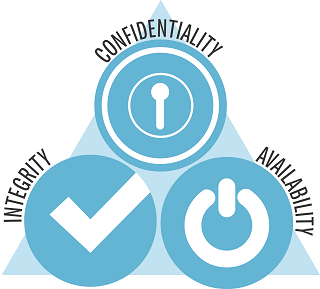
\includegraphics[height=4cm, width=4cm]{figures/cia_triad.png}
	\end{figure}
	\begin{itemize}
		\item การรักษาความลับ (Confidentiality)
		\item การรักษาความครบถ้วนสมบูรณ์ (Integrity)
		\item การรักษาความพร้อมใช้ (Availability)
	\end{itemize}
}

\frame{\frametitle{The CIA triad}
	%\begin{beamercolorbox}[rounded=true,wd=\linewidth]{postit}
	%	Key Concepts
	%\end{beamercolorbox}
	\begin{figure}[!htbp]
		\centering
		
\includegraphics[height=5cm, width=5cm]{figures/ciaaa.png}
	\end{figure}
	\begin{itemize}
		\item การพิสูจน์สิทธิ์ (Authentication)
		\item การกำหนดสิทธิ์ (Authorization)
	\end{itemize}
}

\subsection{ภัยคุกคามและการโจมตี}
\frame{\frametitle{Persisting Threats and Attacks: Experimentation}
	%\begin{beamercolorbox}[rounded=true,wd=\linewidth]{postit}
	%ประเภทของนโยบายฯ
	%\end{beamercolorbox}
	\begin{figure}[!htbp]
		\centering
		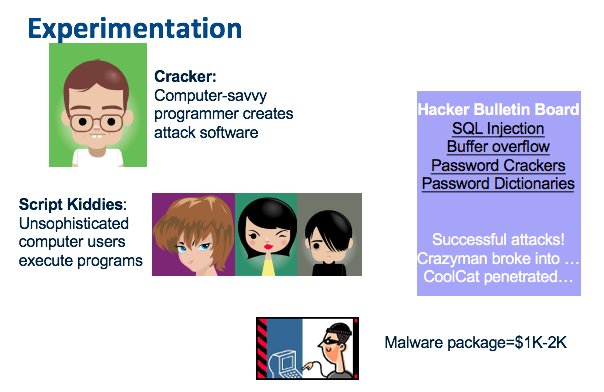
\includegraphics[height=.9\textheight, width=.9\textwidth]{figures/experimentation.png}
	\end{figure}
}

\frame{\frametitle{Persisting Threats and Attacks (Cont.): Malware}
	%\begin{beamercolorbox}[rounded=true,wd=\linewidth]{postit}
	%Regulatory Compliance Policies
	%\end{beamercolorbox}
	\begin{figure}[!htbp]
		\centering
		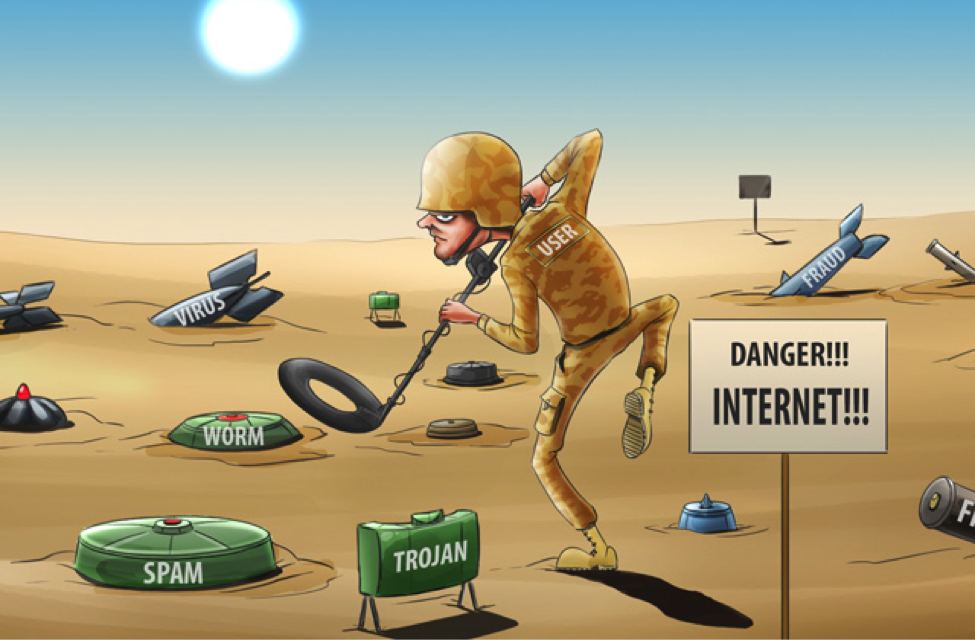
\includegraphics[height=.75\textheight, width=.75\textwidth]{figures/malware.png}
	\end{figure}
}

\frame{\frametitle{Persisting Threats and Attacks (Cont.): Worm}
	%\begin{beamercolorbox}[rounded=true,wd=\linewidth]{postit}
	%Regulatory Compliance Policies
	%\end{beamercolorbox}
	\begin{figure}[!htbp]
		\centering
		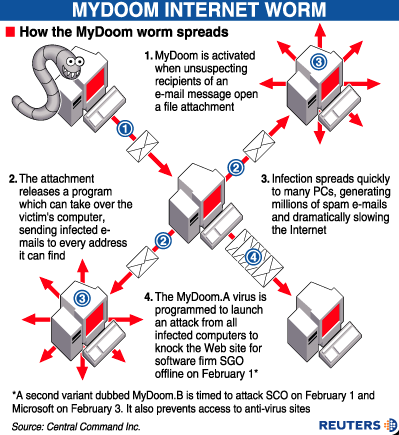
\includegraphics[height=.7\textheight, width=.7\textwidth]{figures/worm.png}
	\end{figure}
	\begin{itemize}
		\item Melissa(2000), I love you (2001), Code red and code red II (2001), My Doom (2003), etc.
	\end{itemize}
}

\frame{\frametitle{Persisting Threats and Attacks (Cont.): Social Engineering}
	%\begin{beamercolorbox}[rounded=true,wd=\linewidth]{postit}
	%Regulatory Compliance Policies
	%\end{beamercolorbox}
	\begin{figure}[!htbp]
		\centering
		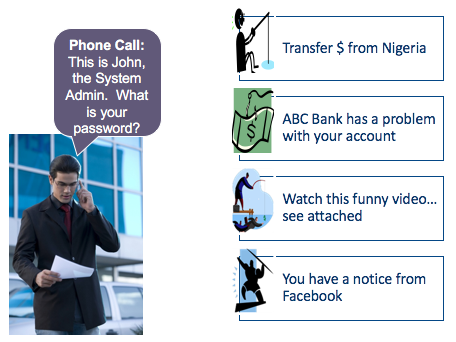
\includegraphics[height=.7\textheight, width=.7\textwidth]{figures/social_engineering.png}
	\end{figure}
	\begin{itemize}
		\item หลอกลวงผู้ใช้งาน, สอบถามพาสเวิร์ด, ฯลฯ
	\end{itemize}
}

\frame{\frametitle{Persisting Threats and Attacks (Cont.): Pharming}
	%\begin{beamercolorbox}[rounded=true,wd=\linewidth]{postit}
	%Regulatory Compliance Policies
	%\end{beamercolorbox}
	\begin{figure}[!htbp]
		\centering
		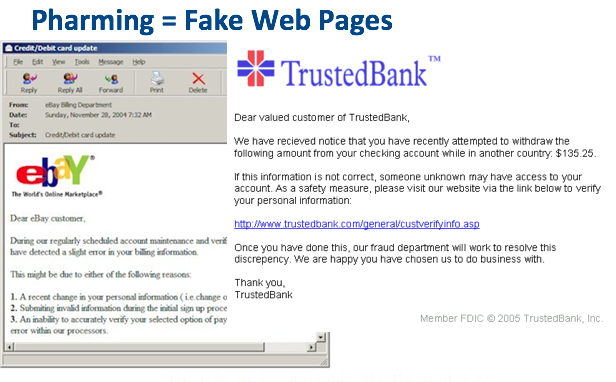
\includegraphics[height=.7\textheight, width=.7\textwidth]{figures/pharming.png}
	\end{figure}
}

\frame{\frametitle{Persisting Threats and Attacks (Cont.): Man-In-The-Middle}
	%\begin{beamercolorbox}[rounded=true,wd=\linewidth]{postit}
	%Regulatory Compliance Policies
	%\end{beamercolorbox}
	\begin{figure}[!htbp]
		\centering
		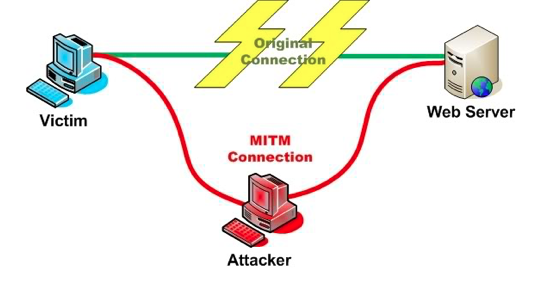
\includegraphics[height=.7\textheight, width=.7\textwidth]{figures/mitm.png}
	\end{figure}
}

\frame{\frametitle{Persisting Threats and Attacks (Cont.): Rootkits}
	%\begin{beamercolorbox}[rounded=true,wd=\linewidth]{postit}
	%Regulatory Compliance Policies
	%\end{beamercolorbox}
	\begin{figure}[!htbp]
		\centering
		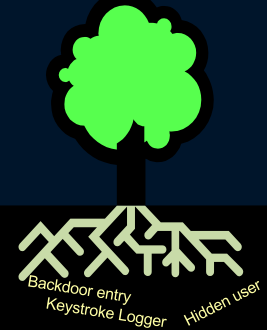
\includegraphics[height=.7\textheight, width=.7\textwidth]{figures/rootkits.png}
	\end{figure}
}

\frame{\frametitle{Persisting Threats and Attacks (Cont.): Botnet}
	%\begin{beamercolorbox}[rounded=true,wd=\linewidth]{postit}
	%Regulatory Compliance Policies
	%\end{beamercolorbox}
	\begin{figure}[!htbp]
		\centering
		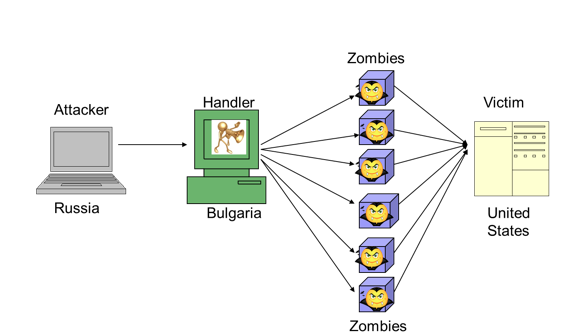
\includegraphics[height=.7\textheight, width=.7\textwidth]{figures/botnet.png}
	\end{figure}
}

\frame{\frametitle{Persisting Threats and Attacks (Cont.): Key logger}
	%\begin{beamercolorbox}[rounded=true,wd=\linewidth]{postit}
	%Regulatory Compliance Policies
	%\end{beamercolorbox}
	\begin{figure}[!htbp]
		\centering
		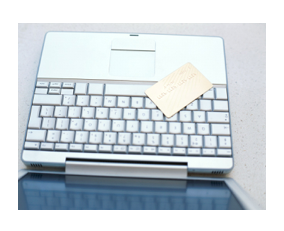
\includegraphics[height=.7\textheight, width=.7\textwidth]{figures/keylogger.png}
	\end{figure}
}

\frame{\frametitle{Persisting Threats and Attacks (Cont.): Trojan}
	%\begin{beamercolorbox}[rounded=true,wd=\linewidth]{postit}
	%Regulatory Compliance Policies
	%\end{beamercolorbox}
	\begin{figure}[!htbp]
		\centering
		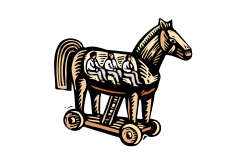
\includegraphics[height=.7\textheight, width=.7\textwidth]{figures/trojan.png}
	\end{figure}
	\centering
}

\frame{\frametitle{Persisting Threats and Attacks (Cont.): War driving}
	%\begin{beamercolorbox}[rounded=true,wd=\linewidth]{postit}
	%Regulatory Compliance Policies
	%\end{beamercolorbox}
	\begin{figure}[!htbp]
		\centering
		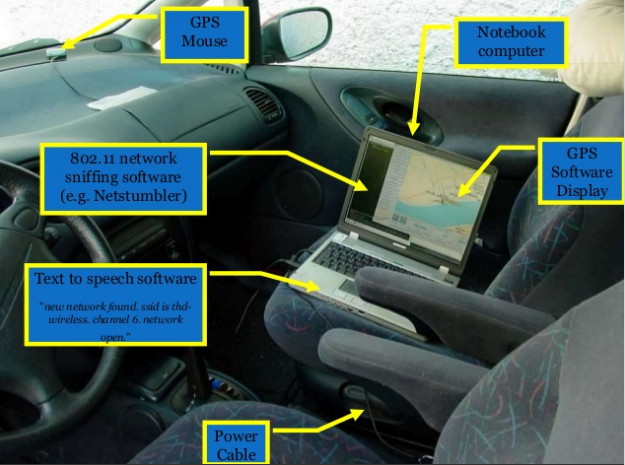
\includegraphics[height=.7\textheight, width=.7\textwidth]{figures/war_driving.png}
	\end{figure}
	\centering
}

\frame{\frametitle{Persisting Threats and Attacks (Cont.): Ransomware}
	%\begin{beamercolorbox}[rounded=true,wd=\linewidth]{postit}
	%Regulatory Compliance Policies
	%\end{beamercolorbox}
	\begin{figure}[!htbp]
		\centering
		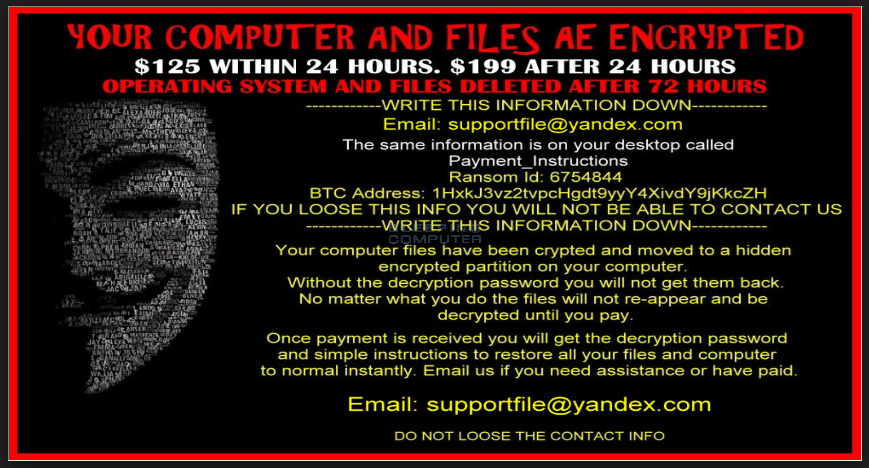
\includegraphics[height=.7\textheight, width=.7\textwidth]{figures/ransomware.png}
	\end{figure}
}

\frame{\frametitle{Persisting Threats and Attacks (Cont.): Password Brute-force}
	%\begin{beamercolorbox}[rounded=true,wd=\linewidth]{postit}
	%Regulatory Compliance Policies
	%\end{beamercolorbox}
	\begin{figure}[!htbp]
		\centering
		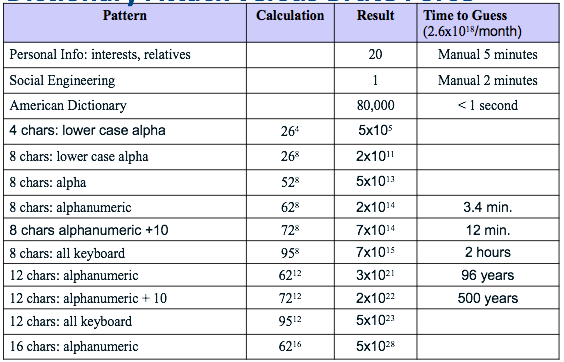
\includegraphics[height=.7\textheight, width=.7\textwidth]{figures/password_cracking.png}
	\end{figure}
	\centering
	ระยะเวลาที่ใช้ในการสุ่มเดาพาสเวิร์ด
}

 
\subsection{Physical Weapons}
\frame{\frametitle{อาวุธเชิงกายภาพ: SCADA}
	%\begin{beamercolorbox}[rounded=true,wd=\linewidth]{postit}
	%Covered topics
	%\end{beamercolorbox}
	%\begin{itemize}
	%	\item 
	%	\item 
	%\end{itemize}
	\centering
	\begin{figure}[!htbp]
		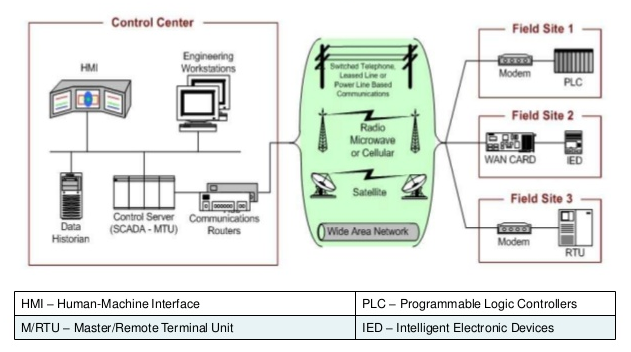
\includegraphics[height=.75\textheight, width=\textwidth]{figures/scada_layout.png}
	\end{figure}
}

\frame{\frametitle{อาวุธเชิงกายภาพ: Electro Magnetic Pulse Weapons}
	%\begin{beamercolorbox}[rounded=true,wd=\linewidth]{postit}
	%Covered topics
	%\end{beamercolorbox}
	%\begin{itemize}
	%	\item 
	%	\item 
	%\end{itemize}
	\centering
	\begin{figure}[!htbp]
		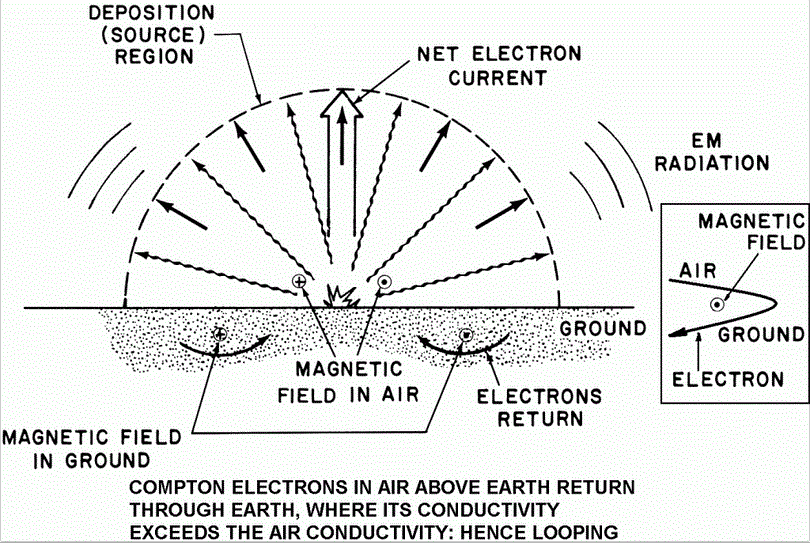
\includegraphics[height=.75\textheight, width=\textwidth]{figures/emp.png}
	\end{figure}
}

\subsection{Psychological Weapons}
\frame{\frametitle{อาวุธเชิงจิตวิทยา}
	%\begin{beamercolorbox}[rounded=true,wd=\linewidth]{postit}
	%Covered topics
	%\end{beamercolorbox}
	%\begin{itemize}
	%	\item 
	%	\item 
	%\end{itemize}
	\centering
	\begin{figure}[!htbp]
		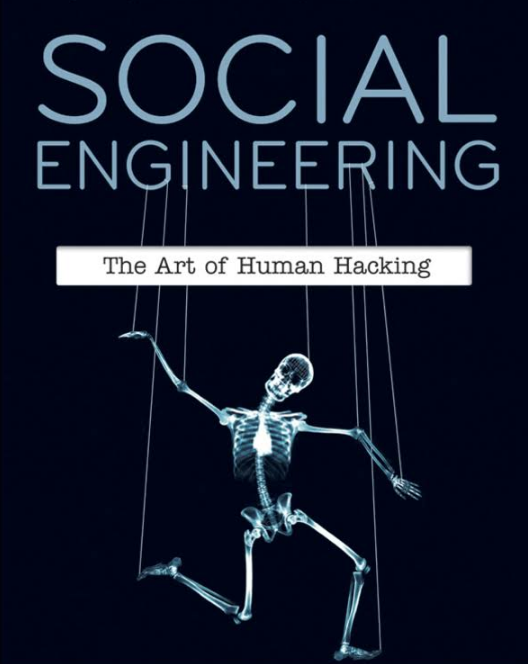
\includegraphics[height=.75\textheight, width=\textwidth]{figures/se.png}
	\end{figure}
}

\subsection{Cyberspace Challenges}
\frame{\frametitle{ความท้าทายของสงครามไซเบอร์}
	%\begin{beamercolorbox}[rounded=true,wd=\linewidth]{postit}
	%Covered topics
	%\end{beamercolorbox}
	\begin{itemize}
		\item \textbf{P} eople = Skills + Organization
		\item \textbf{P} olicy = Organization + Processes
		\item \textbf{T} echnology = Processes + Skills
	\end{itemize}
}

\section{Best Practices}

\frame{\frametitle{คำแนะนำระดับชาติ}
	\begin{itemize}
		\item ปรับตัวและสร้างความตระหนักรู้ในระดับผู้บริหาร
		\item สร้างมาตรการ กฎหมาย และความร่วมมือกับชาติพันธมิตร
		\item พัฒนาโครงสร้างพื้นฐานที่เกี่ยวข้อง (PPT)
	\end{itemize}
}


\frame{\frametitle{คำแนะนำหน่วยงานความมั่นคง}
	%\begin{beamercolorbox}[rounded=true,wd=\linewidth]{postit}
	%	ประเภทของนโยบายฯ
	%\end{beamercolorbox}
	\begin{itemize}
		\item บังคับใช้มาตรการที่จำเป็นเพื่อรักษาความมั่นคงปลอดภัย
		\item นำแนวทางการบริหารจัดการความมั่นคงปลอดภัยมาประยุกต์ใช้ (ISO2700x)
		\item หมั่นตรวจสอบความมั่นคงปลอดภัยตามแนวทางที่กำหนดขึ้น
		\item ประสานความร่วมมือกับหน่วยงานที่เกี่ยวข้อง (ThaiCert)
	\end{itemize}
}

\frame{\frametitle{คำแนะนำหน่วยงานความมั่นคง}
	%\begin{beamercolorbox}[rounded=true,wd=\linewidth]{postit}
	%	ประเภทของนโยบายฯ
	%\end{beamercolorbox}
	\centering
	\begin{figure}[!htbp]
		\centering
		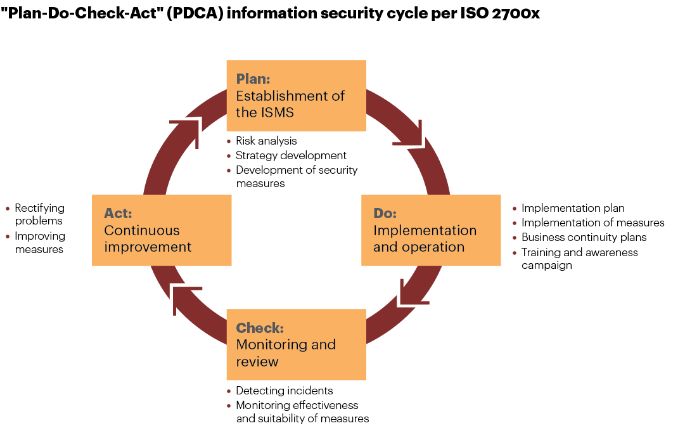
\includegraphics[height=\textheight, width=\textwidth]{figures/pdca.png}
	\end{figure}

}

\frame{\frametitle{คำแนะนำในระดับปัจเจกบุคคล}
	%\begin{beamercolorbox}[rounded=true,wd=\linewidth]{postit}
	%	ประเภทของนโยบายฯ
	%\end{beamercolorbox}
	\begin{itemize}
		\item ตระหนักรู้ถึงภัยคุกคามทางไซเบอร์ และใช้เทคโนโลยีอย่างมั่นคงปลอดภัย
		\item ติดตั้งซอฟต์แวร์ตรวจจับไวรัส มัลแวร์
		\item ตระหนักรู้ถึงการโจมตีแบบวิศวกรรมเชิงสังคมและมัลแมร์
		\begin{itemize}
			\item ไม่เปิดไฟล์ที่แนบมากับอีเมล์ที่ไม่น่าไว้วางใจ
			\item เปิด ดาว์นโหลดและซอฟต์แวร์จากแหล่งที่น่าเชื่อถือ
			\item อัปเดตระบบปฏิบัติการให้ทันสมัยอยู่เสมอ
			\item หลีกเลี่ยงการใช้พาสเวิร์ดที่ง่ายต่อการคาดเดา
			\item สำรองข้อมูลอยู่เสมอๆ เปลี่ยนพาสเวิร์ดบ่อยๆ
		\end{itemize}
	\end{itemize}
}

\section{Question and Discussion}
\frame{\frametitle{Question and Discussion}
\begin{figure}[!htbp]
    \centering
    
\includegraphics[height=4cm, width=4cm]{figures/q_n_d.jpg}
\end{figure}
\centering 
โทรศัพท์มือถือ และเครื่องคอมพิวเตอร์ที่ท่านใช้...มีความมั่นคงปลอดภัยหรือไม่???
}

\frame{\frametitle{References}
	\begin{figure}[!htbp]
		\centering
		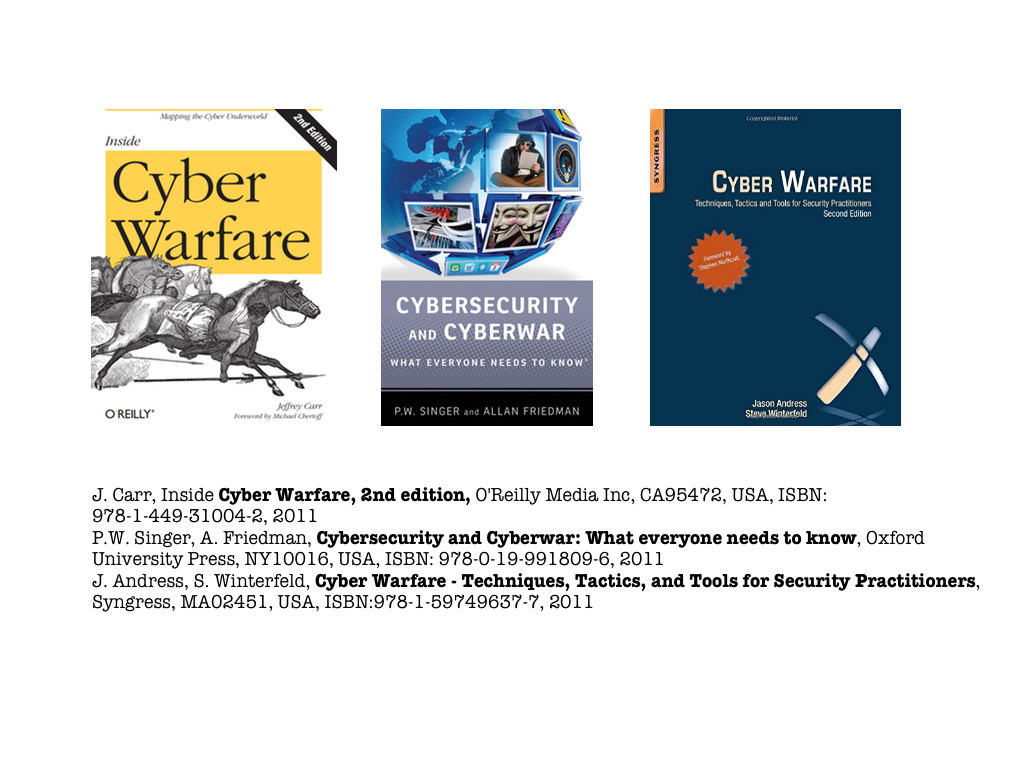
\includegraphics[height=\textheight, width=\textwidth]{figures/reference.png}
	\end{figure}
	\centering 
}

\end{document}